\chapter{Used data}

\section{Raw data intuition}

The raw input into any of our models is the protein's 3D structure. This is represented by a point cloud on the protein's surface. Each point has a feature vector attached, which represents the chemical properties of the given accessible surface patch. Each point also has a ligand-binding class, which the model is used to train and then predict. These can be seen in the figure~\ref{fig:data_point_cloud}.

\begin{figure}
    \centering
    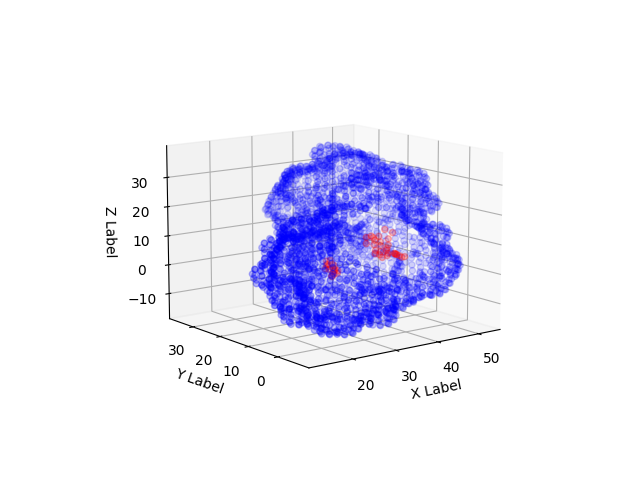
\includegraphics[width=1\linewidth]{img/protein.png}
    \caption{Point cloud with 2 highlighted ligand-binding sites}
    \label{fig:data_point_cloud}
\end{figure}

In the implementation, these points are represented as tabular data, with three columns representing the X, Y, and Z axis, respectively. From this data, the point cloud can be recreated.

\section{Features}

\section{Surroundings extraction}

For the following models, we need to have features for the site's surroundings and the features logged for it.

To achieve this, we run a simple quadratic algorithm for finding the k nearest neighbors. Then, we append their features to the original ones. We use these features instead of the original ones for the following algorithms.
